\section{Classifieur 1 : profils et classifieur par distance euclidienne minimum}

Listes des fonctions mentionnées dans cette section : \textit{extractprofile}, \textit{computepdistances}, \textit{learningclassifier1}, \textit{decisionclassifier1}.

\subsection{Principe et implémentation}

Ce premier classifieur vise à déterminer un chiffre en fonction de ses profils gauche et droit. La première étape consiste à extraire ces profils du chiffre, puis de décider de la nature de la classe de ces profils, grâce à la distance euclidienne minimum.

Pour pouvoir effectuer un classement des profils, il est nécessaire de passer par une phase d'apprentissage, afin d'obtenir une base de profils de référence. Il est alors possible de comparer les profils de référence et ceux récupérés sur le chiffre souhaitant être lu.

\subsubsection{Fonctions utilisées}

\textit{extractprofile( base, d ) : profile}\\
\begin{itemize}
	\item[\textbf{Entrées :}] \textbf{base} est l'image du rectangle contenant le chiffre à lire, grâce au pré-traitement effectué. \textbf{d} est le nombre de composantes d'un profil
	\item[\textbf{Sortie :}] \textbf{profile} est le vecteur contenant les deux profils (gauche et droit), de dimension $d\times2$
\end{itemize}
Pour un chiffre donné, on découpe dans celui-ci $d$ lignes équidistantes les unes des autres, sur lesquelles les profils vont être lus. Pour chaque ligne, son profil gauche ainsi que son droit sont alors relevés. Le profil est alors normalisé, pour qu'il n'y ait aucune incohérence entre chaque chiffre et la base de référence.\\

\textit{computepdistances( centerslearning, vectordistance ) : pbelonging}\\
\begin{itemize}
	\item[\textbf{Entrées : }] \textbf{conterslearning} contient les centres d'une classe, obtenus lors de la phase d'apprentissage. \textbf{vectordistance} contient les centres de la classe à tester.
	\item[\textbf{Sortie :}] \textbf{pbelonging} contient les probabilités d'appartenance de la classe à tester dans la classe d'apprentissage
\end{itemize}
Il s'agit ici de calculer la probabilité pour une classe précise, suivant la formule suivante :
$$p(\omega_i/x) = \frac{exp(-d(x,\omega_i)}{\sum_{j=0}^9 exp(-d(x, \omega_j))}$$

\subsubsection{Phase d'apprentissage}

\textit{learningclassifier1( rectangleslearning, learningimage, d ) : vectordistancelearning}\\
\begin{itemize}
	\item[\textbf{Entrées :}] \textbf{rectangleslearning} correspond aux rectangles déterminés précédemment permettant d'isoler chaque chiffre sur l'image d'apprentissage. \textbf{learningimage} est l'image d'apprentissage, et \textbf{d} le nombre de composantes pour un profil
	\item[\textbf{Sortie :}] \textbf{vectordistancelearning} contient l'ensemble des centres des profils pour chaque chiffre
\end{itemize}
Grâce à \textit{extractprofile}, un profil est déterminé pour chaque chiffre. Les vecteurs déterminant les profils récupérés, la moyenne des centres pour chaque classe est calculé, à l'aide de \textit{mean}. Ces résultats sont sauvegardés pour faire office de base de référence. 

\subsubsection{Phase de décision}

\textit{decisionclassifier1( rectangles, image, vectordistancelearning, d ) : pbelonging}\\
\begin{itemize}
	\item[\textbf{Entrées :}] \textbf{rectangles} correspond aux rectangles déterminés précédemment permettant d'isoler chaque chiffre sur l'image à lire. \textbf{image} est l'image à lire. \textbf{vectordistancelearning} est la base de référence déterminée dans la phase d'apprentissage. \textbf{d} est le nombre de composantes pour un profil
	\item[\textbf{Sortie :}] \textbf{pbelonging} contient les probabilités d'appartenance de chaque chiffre par rapport à l'ensemble des classes d'apprentissage
\end{itemize}
Le fonctionnement est semblable à la phase d'apprentissage. Il y a d'abord une extraction du profil pour chaque chiffre, puis la probabilité d'appartenance à chaque classe en fonction de ses centres est calculée grâce à \textit{computepdistances}.

\subsection{Analyse et conclusion}
\subsubsection{Evaluation des performances}
La figure~\ref{fig:proba1} indique la probabilité, pour chaque chiffre lu, d'appartenir à telle classe de chiffre. De gauche à droite, les classes vont de 0 à 9. Une probabilité élevée indique une plus forte chance pour un chiffre de se trouver dans cette classe.

\begin{figure}[hm]
	\begin{center}
		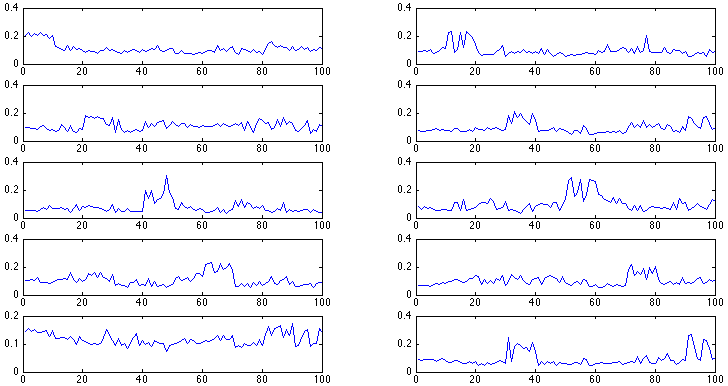
\includegraphics[width=\textwidth]{img/20-pbelonging1.png}
	\end{center}
	\caption{Probabilité de classe pour chaque chiffre}
	\label{fig:proba1}
\end{figure}

On peut remarquer que le classifieur repère des tendances dans les chiffres analysés. Si l'on prend par exemple la classe 0, un pic se forme là où il y a bien des 0 sur l'échantillon à analyser (figure~\ref{fig:proba102}, gauche). Cependant, sur certains chiffres, comme la classe 2 (figure~\ref{fig:proba102}, droite), il est difficile d'obtenir un résultat convenable partout. Ici, l'analyse des chiffres 8 (entre 80 et 90) amène à penser qu'il peut s'agir de la classe 2, car les probabilités sont aussi hautes que lorsqu'il s'agissait de la classe 2 elle-même.

\begin{figure}[hm]
	\begin{center}
		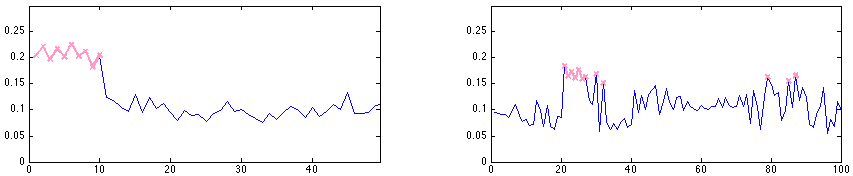
\includegraphics[width=\textwidth]{img/21-pbelonging1-more.png}
	\end{center}
	\caption{Probabilité pour les classes 0 et 2}
	\label{fig:proba102}
\end{figure}

Cette méthode aide donc à obtenir un premier classement, mais n'est pas tout le temps précise. Elle nécessite l'apport d'un classifieur supplémentaire.

\subsubsection{Variation de la valeur $d$}
Le paramètre qu'il est possible de varier ici est $d$, qui correspond à la taille du vecteur contenant les profils gauches et droits d'un chiffre. Ainsi, pour une valeur plus élevée de $d$, environ 10 ou plus, ce premier classifieur permet d'obtenir des résultats à 80\% satisfaisants. Par contre, des valeurs moins importantes que 5 ne permettent pas d'avoir un classifieur correct, puisque le taux de confiance se situe en-dessous de 60\%.

\begin{figure}[hm]
	\begin{center}
		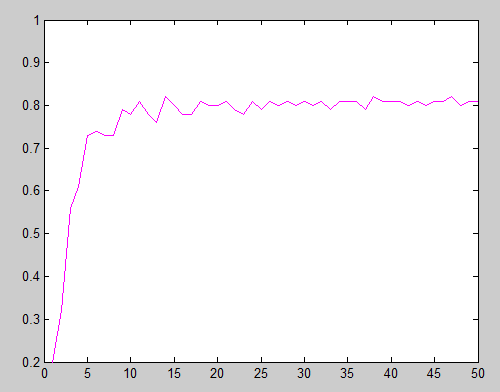
\includegraphics[width=0.6\textwidth]{img/22-influence-d.png}
	\end{center}
	\caption{Influence de $d$}
	\label{fig:probad}
\end{figure}

Il est donc raisonnable de posséder un nombre de mesure par profil au delà d'un seuil, à savoir ici 10 ou plus. La figure~\ref{fig:proba1d} fournit des résultats plus contrastés que ceux relevés dans la figure~\ref{fig:proba1}, pour $d = 15$. Pour certains chiffres, il y a même une certitude de quasiment 100\% qu'il s'agit de ceux-ci.

\begin{figure}[hm]
	\begin{center}
		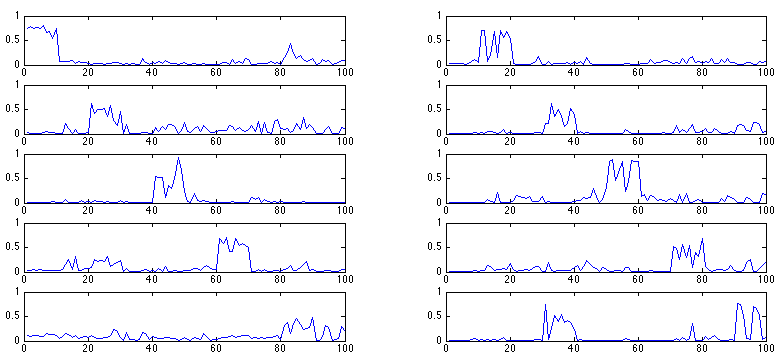
\includegraphics[width=\textwidth]{img/23-pbelonging1-influence-d.png}
	\end{center}
	\caption{Probabilité de classe pour $d = 15$}
	\label{fig:proba1d}
\end{figure}
